\documentclass[a4paper]{article} 
\addtolength{\hoffset}{-2.25cm}
\addtolength{\textwidth}{4.5cm}
\addtolength{\voffset}{-3.25cm}
\addtolength{\textheight}{5cm}
\setlength{\parskip}{0pt}
\setlength{\parindent}{0in}

\usepackage[square,sort,comma,numbers]{natbib}
\usepackage{blindtext} % Package to generate dummy text
\usepackage{charter} % Use the Charter font
\usepackage[utf8]{inputenc} % Use UTF-8 encoding
\usepackage{microtype} % Slightly tweak font spacing for aesthetics
\usepackage{amsthm, amsmath, amssymb} % Mathematical typesetting
\usepackage{float} % Improved interface for floating objects
\usepackage{hyperref} % For hyperlinks in the PDF
\usepackage{graphicx, multicol} % Enhanced support for graphics
\usepackage{xcolor} % Driver-independent color extensions
\usepackage{pseudocode} % Environment for specifying algorithms in a natural way
\usepackage[mmddyy]{datetime} % Uses YEAR-MONTH-DAY format for dates

\usepackage{fancyhdr} % Headers and footers
\pagestyle{fancy} % All pages have headers and footers
\fancyhead{}\renewcommand{\headrulewidth}{0pt} % Blank out the default header
\fancyfoot[L]{} % Custom footer text
\fancyfoot[C]{} % Custom footer text
\fancyfoot[R]{\thepage} % Custom footer text
\newcommand{\note}[1]{\marginpar{\scriptsize \textcolor{red}{#1}}} % Enables comments in red on margin

\DeclareMathOperator*{\argmin}{arg\,min}

%----------------------------------------------------------------------------------------


%-------------------------------
%	TITLE VARIABLES (identify your work!)
%-------------------------------

\newcommand{\yourname}{Balthazar Neveu | Jamy Lafenetre}
\newcommand{\youremail}{balthazarneveu@gmail.com | jamy.lafenetre@ens-paris-saclay.fr}
\newcommand{\assignmentnumber}{2}

\begin{document}

%-------------------------------
%	TITLE SECTION (do not modify unless you really need to)
%-------------------------------
\fancyhead[C]{}
\hrule \medskip
\begin{minipage}{0.295\textwidth} 
\raggedright
\footnotesize
\yourname \hfill\\
\youremail
\end{minipage}
\begin{minipage}{0.4\textwidth} 
\centering 
\large 
Lab session \# \assignmentnumber\\ 
\normalsize 
NPM 2024\\ 
\end{minipage}
\begin{minipage}{0.295\textwidth} 
\raggedleft
\today\hfill\\
\end{minipage}
\medskip\hrule 
\bigskip




%-------------------------------
%	ASSIGNMENT CONTENT (add your responses)
%-------------------------------


\section*{Question 1: ICP}
\begin{figure}[ht]
    \centering
    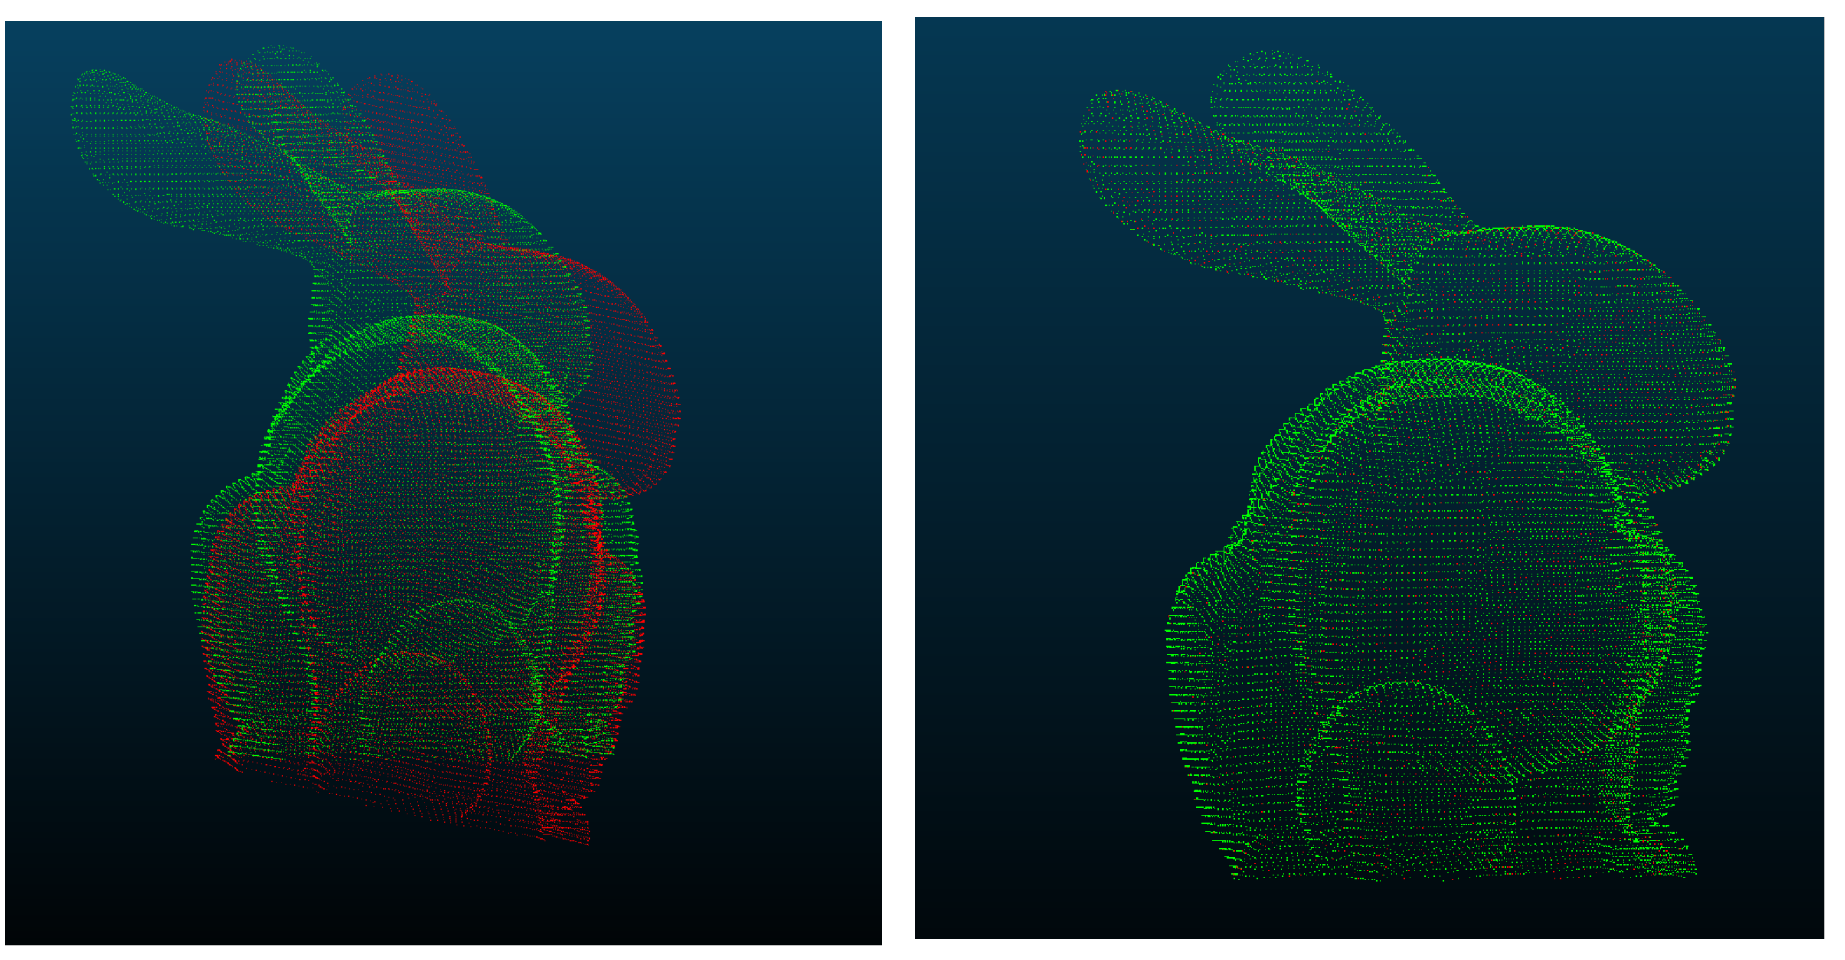
\includegraphics[width=0.8\linewidth]{figures/bunny_icp_cloud_compare.png}
    \caption{Left: reference cloud in green (template to match), misaligned candidate cloud in red. Right: After ICP alignment in Cloud Compare, $\text{RMSE}=7.2. 10^{-8}$}
    \label{fig:CC_alignment_ok}
\end{figure}

\begin{figure}[ht]
    \centering
    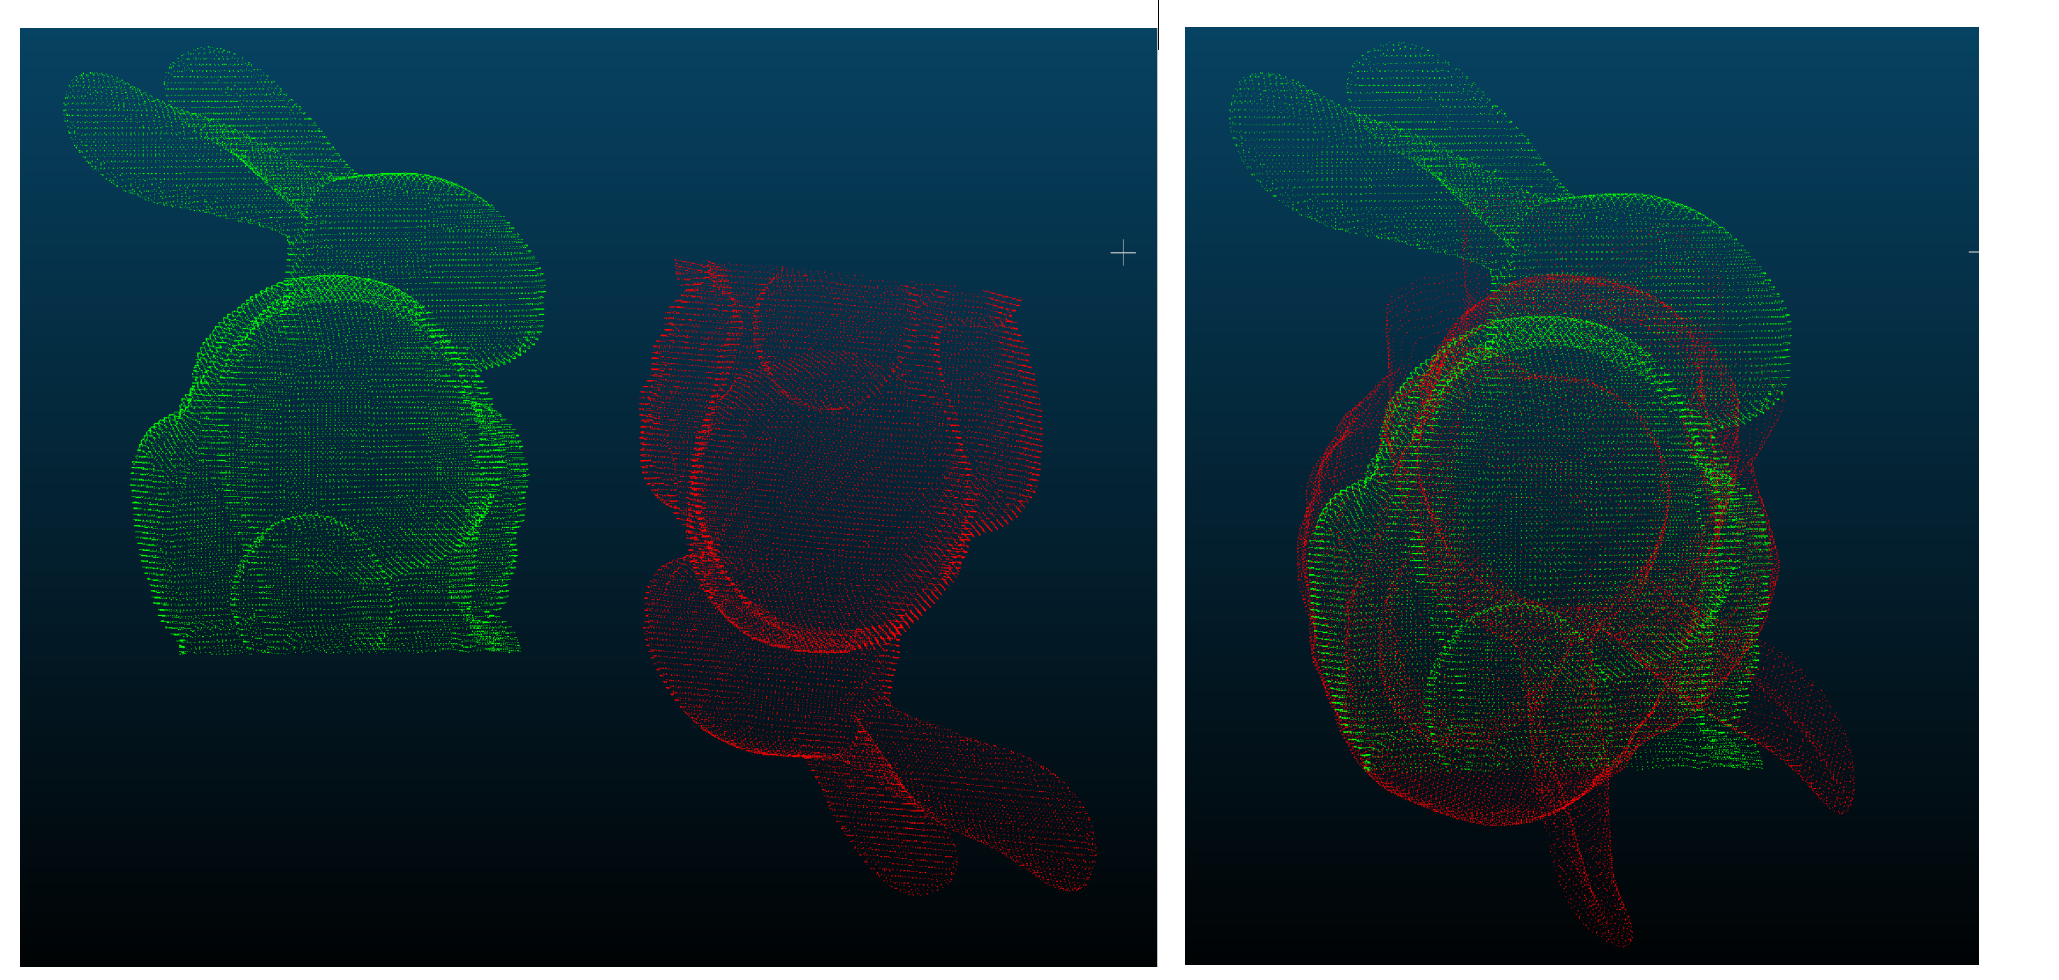
\includegraphics[width=0.8\linewidth]{figures/bunny_icp_upside_down_cloud_compare.png}
    \caption{Left: reference cloud in green (template to match), misaligned candidate cloud in red (upside down initialization). 
    Right: After ICP alignment in Cloud Compare, root mean squared error $\text{RMSE}=0.013$}
    \label{fig:CC_alignment_nok}
\end{figure}

The ICP algorithm is very sensitive to initialization. For the bunny example (same geometry without noise), two different initializations provide very different results.
Figure ~\ref{fig:CC_alignment_ok} shows a nearly perfect alignment, while Figure ~\ref{fig:CC_alignment_nok} shows a bad alignment likely due to getting stuck in a local minimum.

\pagebreak

\begin{figure}[ht]
    \centering
    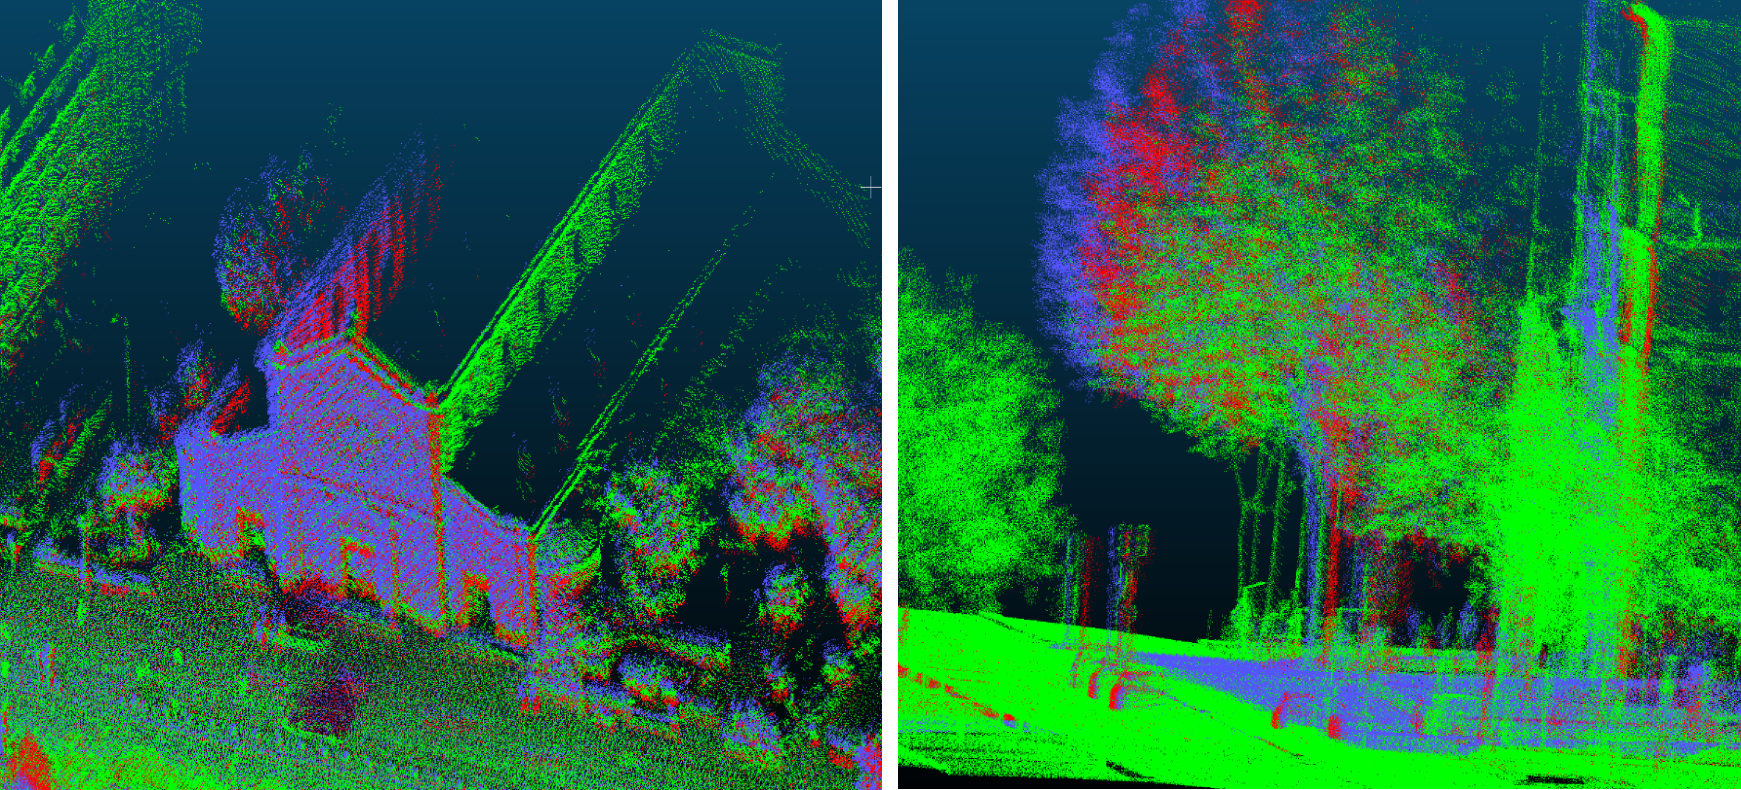
\includegraphics[width=0.8\linewidth]{figures/notre_dame_des_champs_registration.png}
    \caption{Reference cloud in green - the largest cloud, misaligned candidate cloud in blue and ICP registration result in red $\text{RMSE}=1.39$. The registration is off by more than a meter on average, but the scene contains objects that moved between the scans: an outlier removal could strongly enhance the result of the registration algorithm.}
    \label{fig:CC_notredame}
\end{figure}

The estimated transformation matrix is quite close to the identity matrix since the misalignment was quite small. It seems like most of the misalignment source came from the ground not being perfectly aligned (the blue ground is not horizontal in figure ~\ref{fig:CC_notredame_z})
\begin{verbatim}
  Transformation matrix - Scale: fixed (1.0)
  0.999	0.008	0.032	6.017
  -0.010	0.998	0.060	-8.688
  -0.031	-0.060	0.998	-67.759
  0.000	0.000	0.000	1.000
\end{verbatim}

\begin{figure}[ht]
    \centering
    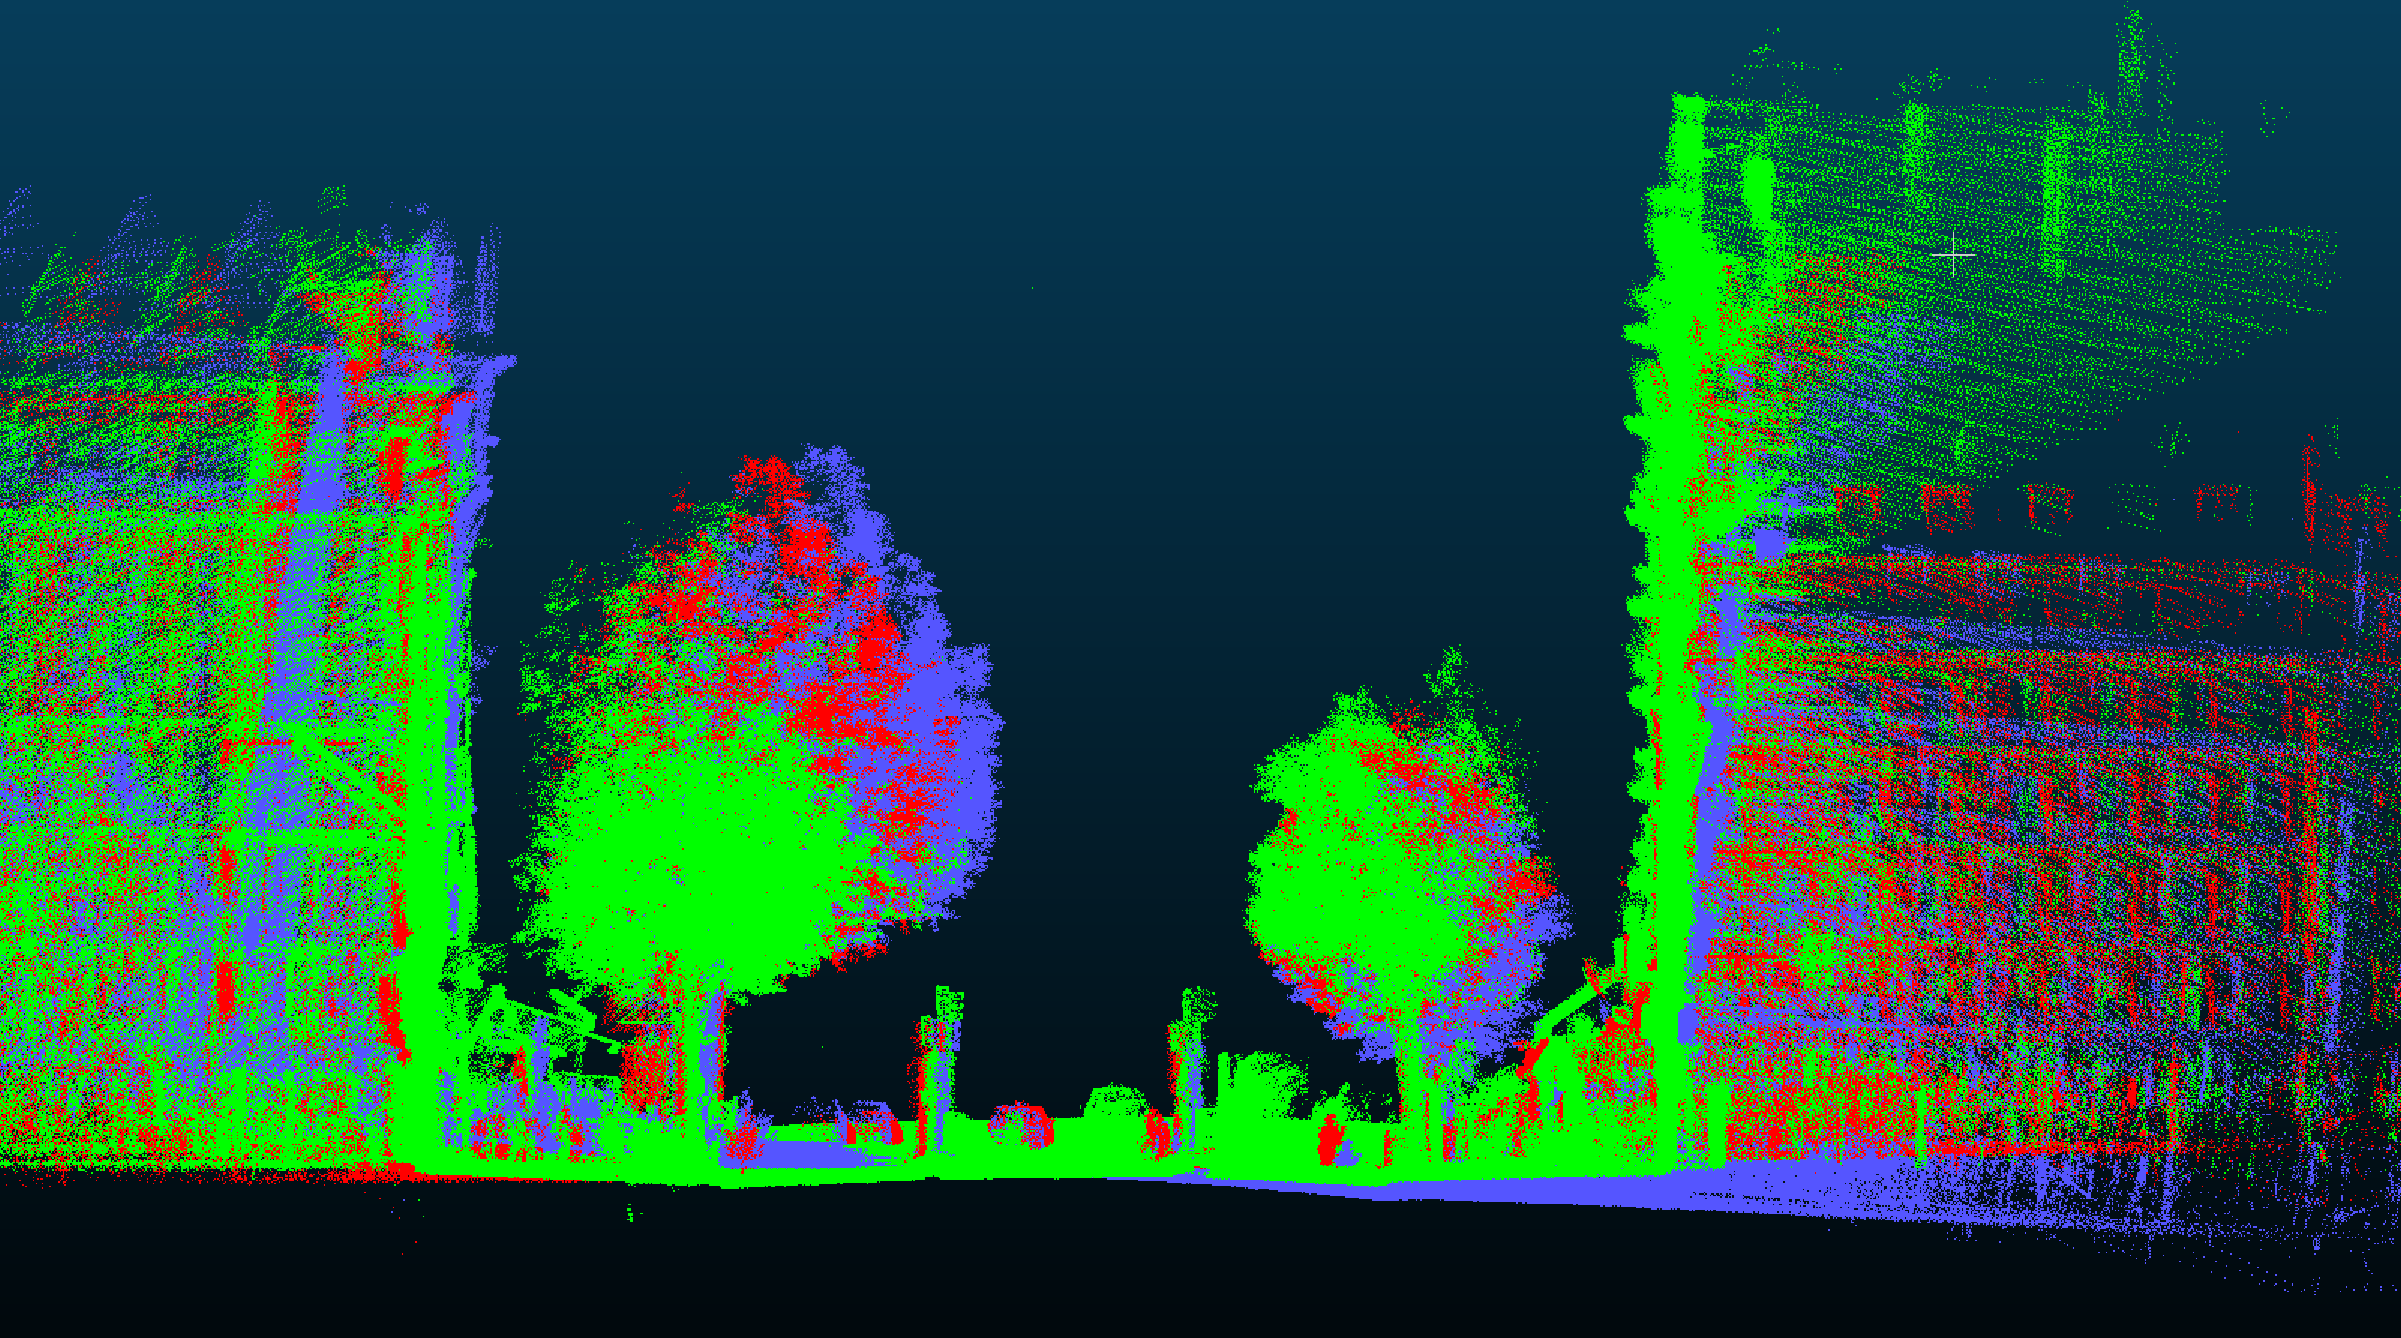
\includegraphics[width=0.8\linewidth]{figures/notre_dame_des_champs_registration_rotation.png}
    \caption{Most of the misalignment seem to have been on the Z axis - ground is not horizontal in the blue misaligned scene.}
    \label{fig:CC_notredame_z}
\end{figure}
\textbf{We use the largest cloud as reference cloud (Notre dame des champs 1).} It seems more natural as the small candidate cloud can potentially match all its points to the bigger reference cloud (this does not work the other way around).

\pagebreak

\section*{Question 2: Rigid transformation estimation}
\begin{itemize}
  \item We are dealing with 2 pre-matched point clouds without any noise.
  \item We obtain a perfect alignment $\text{RMS} = 0$.
It works perfectly because the input points are perfectly matching (no noise or sampling disparity) and we use a \textbf{closed form solution} for the rigid transformation estimation.
  \item ICP struggles because of a bad initialization and gets stuck in a local minimum (a good estimation of the translation could still be estimated, see figure \ref{fig:CC_alignment_nok}).
\end{itemize}


For the real raw scene "Notre Dame des champs", we do not have a matching between points (and we don't have the same amount of points.). One would have to first find matches, which is the purpose of ICP studied in the next section.

\pagebreak
\section*{Questions 3 and 4: ICP convergence}
\subsection*{2D toy example}
\begin{figure}[ht]
  \centering
  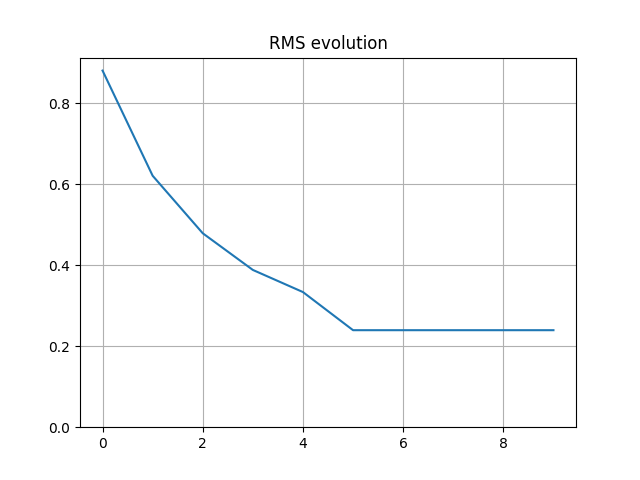
\includegraphics[width=0.4\linewidth]{figures/icp_2d_toy_example.png}
  \caption{ICP 2D toy example:  RMS error as a function of the number of iterations.}
  \label{fig:icp_toy_convergence}
\end{figure}


After the fifth iteration, the algorithm finished converging with an $\text{RMSE}$ of $0.2395$ as seen in \ref{fig:icp_toy_convergence}. It cannot reach zero because both clouds have been sampled at different positions, see the zoom in figure \ref{fig:icp_toy_convergence_zoom}.

In the 2D toy example, we are matching a large reference point cloud (in blue) and a candidate smaller point cloud (in orange). 
ICP will find the best rotation and 2D translations (3 degrees of freedom) and find the matches between the two point clouds (the whole candidate cloud with a subset of the reference cloud).
Matches are shown in green in figure \ref{fig:icp_toy}.

\begin{figure}[ht]
  \centering
  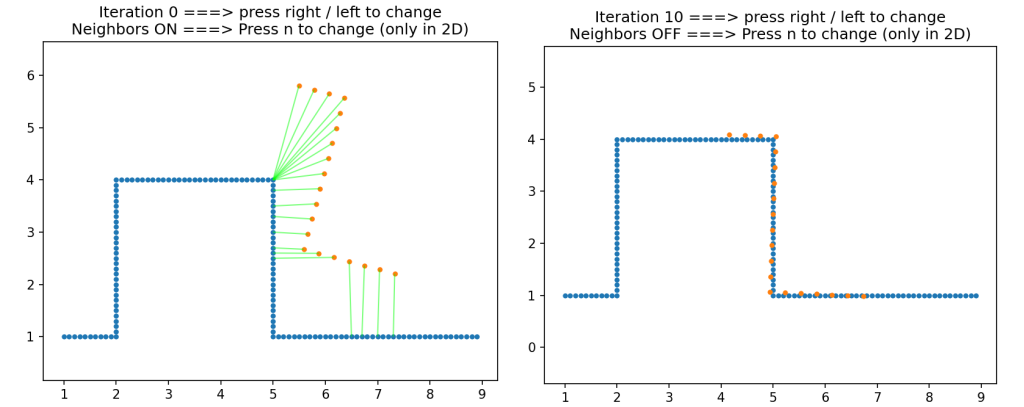
\includegraphics[width=0.8\linewidth]{figures/icp_convergence.png}
  \caption{ICP 2D toy example: nearest neighbor search pairs (matching in green). Initialization on the left, end of convergence on the right side.}
  \label{fig:icp_toy}
\end{figure}

\begin{figure}[ht]
  \centering
  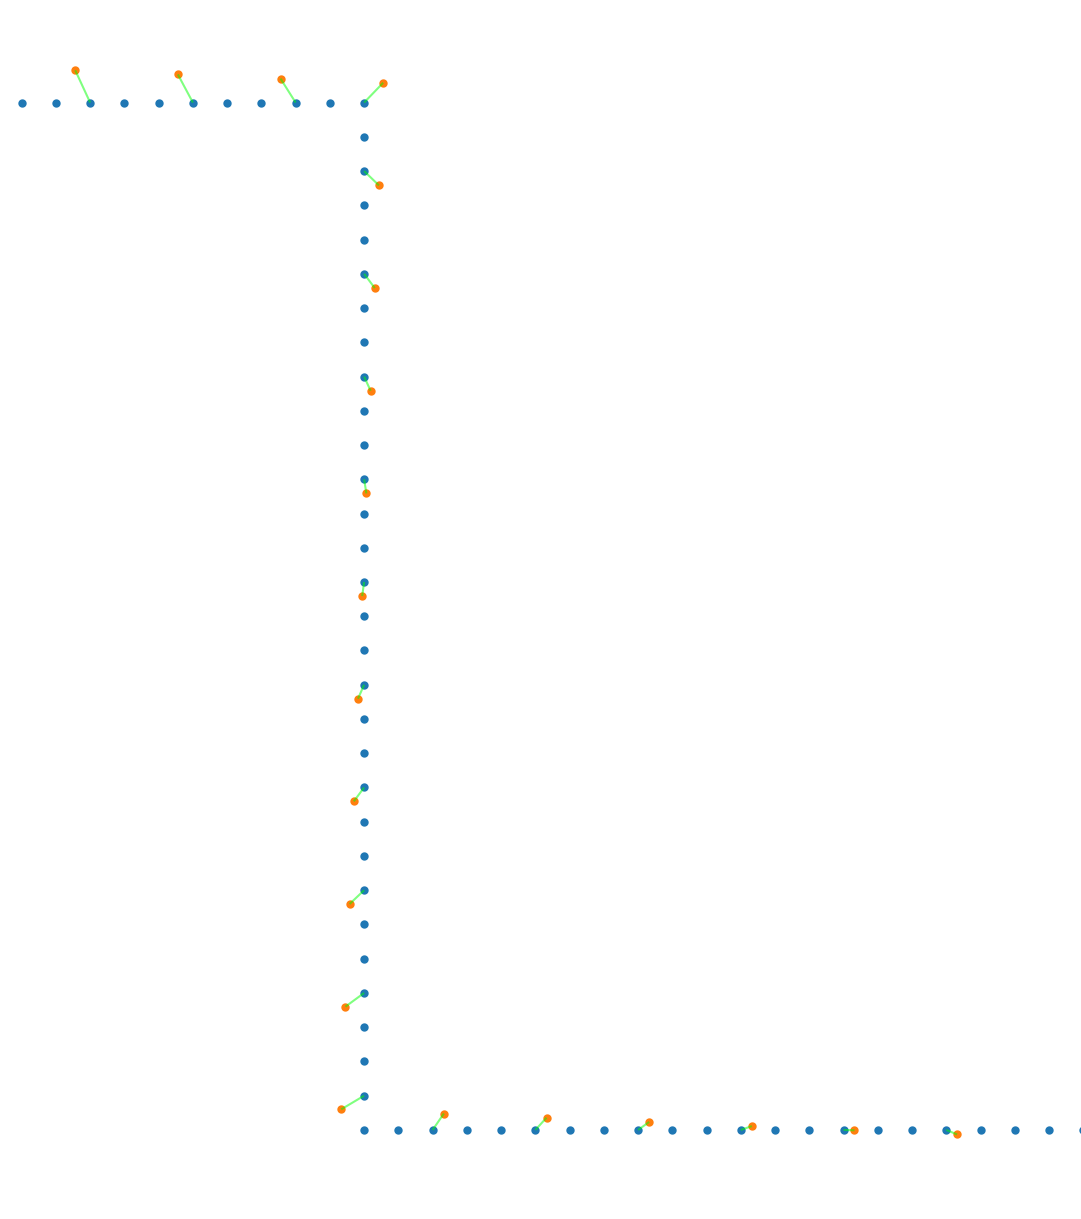
\includegraphics[width=0.4\linewidth]{figures/icp_2d_toy_example_zoom.png}
  \caption{Zoom on the registered 2D point clouds after the fifth iteration. The algorithm has converged and the pointwise distances can indeed hardly be smaller. Yet, as highlighted by the Gestalt theory, the nature of our brain tricks us into extrapolating shapes and to consider that the alignment could be improved.}
  \label{fig:icp_toy_convergence_zoom}
\end{figure}

\pagebreak
\subsection*{3D ICP}
Just like we had noticed in the rigid alignment, the two bunnies can be perfectly aligned ($RMSE=0$). There is \textbf{a convergence acceleration} near the end, although the changes are hardly noticeable visually between steps 15 to 18 (\textit{Visualizing the rotation and translation errors would probably show that the convergence was almost finished earlier.})
\begin{figure}[ht]
  \centering
  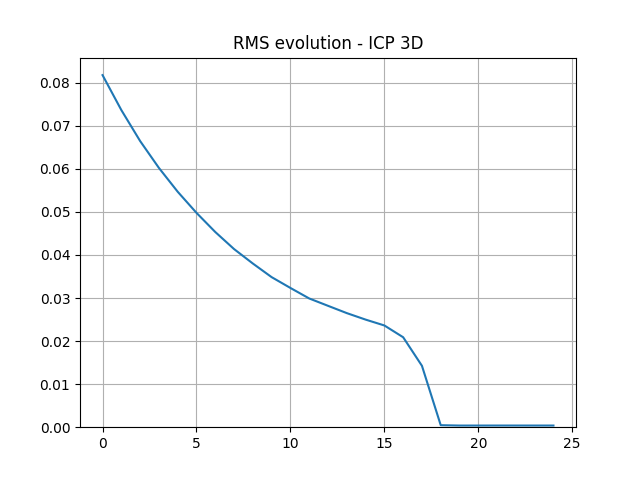
\includegraphics[width=0.8\linewidth]{figures/icp3d_rms.png}
  \caption{Evolution of the RMSE using the ICP algotithm on a 3D example.}
  \label{fig:icp_3D}
\end{figure}

\begin{figure}[ht]
  \centering
  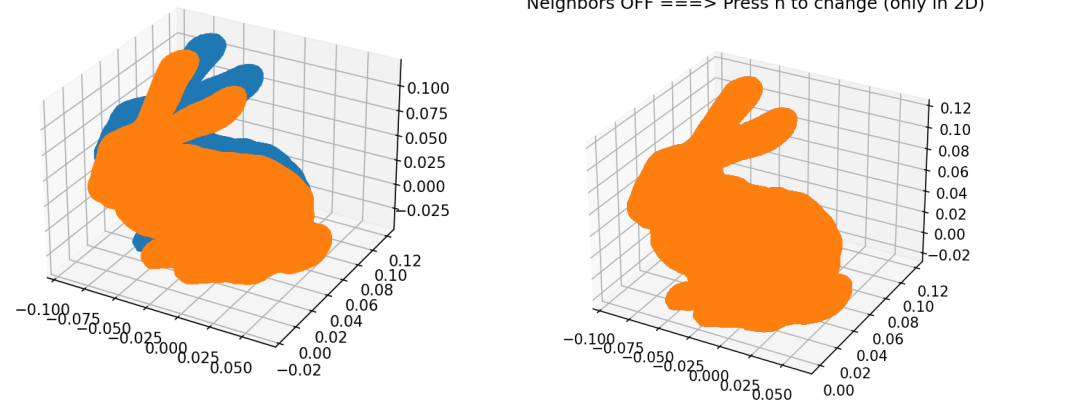
\includegraphics[width=0.8\linewidth]{figures/icp3d_convergence.png}
  \caption{ICP 3D example: Initialization on the left, end of convergence on the right side.}
  \label{fig:icp_3D}
\end{figure}





\pagebreak

\section*{Bonus question: ICP on large point clouds}
We are able to align the 2 large point clouds in approximately 5 seconds with an error of roughly 50cm. Building the KD tree takes most of the time (4.6s). The error seems to slightly increase, one should therefore keep an history of the transformations to keep the best one. However, it requires to compute the RMSE with a lot of points. Whether using 1k or 10k points, the minimum RMSE is not so different but the approximation of the RMSE on the current randomly selected points is quite noisy.
Using 10k points provides less noisy RMSE estimates (see figure \ref{fig:real_scene_icp}) but takes longer to converge (see figure \ref{fig:real_scene_icp_true}). A viable solution is to start iterating with few points, then gradually increase the number of samples. It allows to refine the estimate, as well as stabilizing the variance of the empirical RMSE in order for the stopping condition to be more reliable.

\begin{figure}[H]
  \centering
  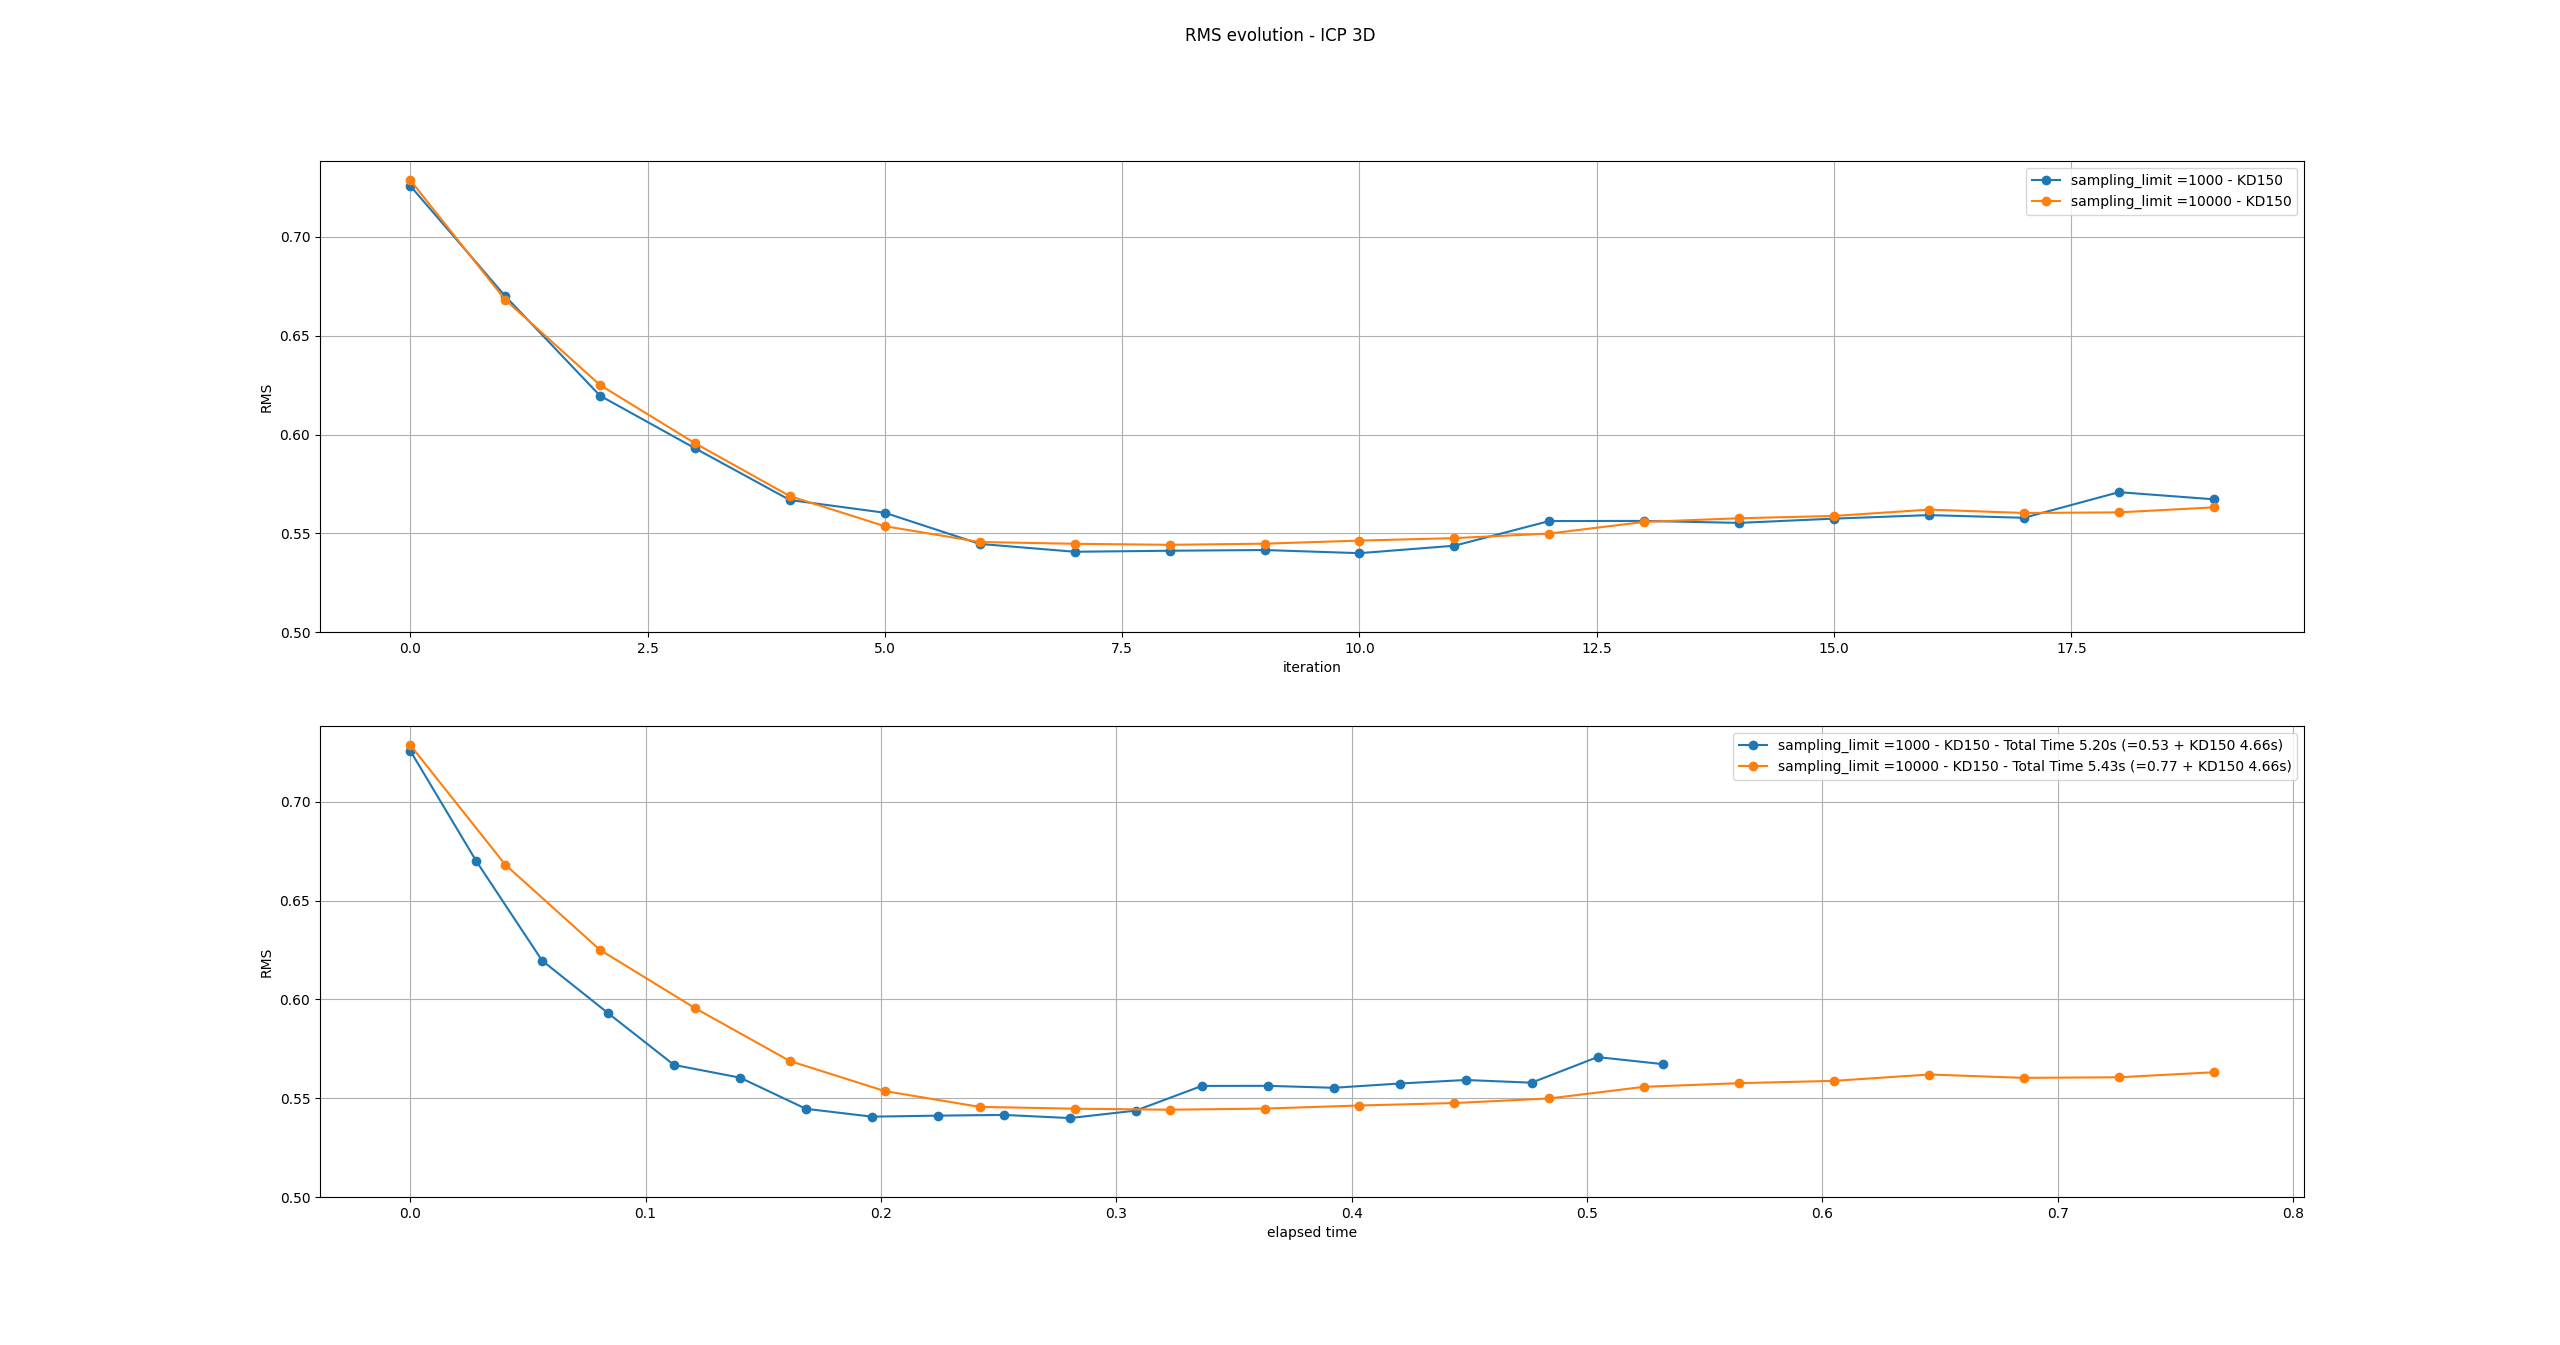
\includegraphics[width=1.\linewidth]{figures/RMS_random_sampling_limit_1k_vs_10k.png}
  \caption{True RMSE (estimated over the whole point cloud) when doing ICP over a random selection of 1000 and 10.000 matched points.}
  \label{fig:real_scene_icp_true}
\end{figure}

% If we use a lot of points in the nearest neighbor search, it is more computationally expensive and looks more accurate.
% Using less points (1000 points to match at each iteration) is faster but the criterion to decide if the algorithm has converged is definitely not as good, to actually know if the algorithm has converged, we would need to compute the RMS error on way more points. This can be seen in figure \ref* {fig:real_scene_icp}


\begin{figure}[H]
  \centering
  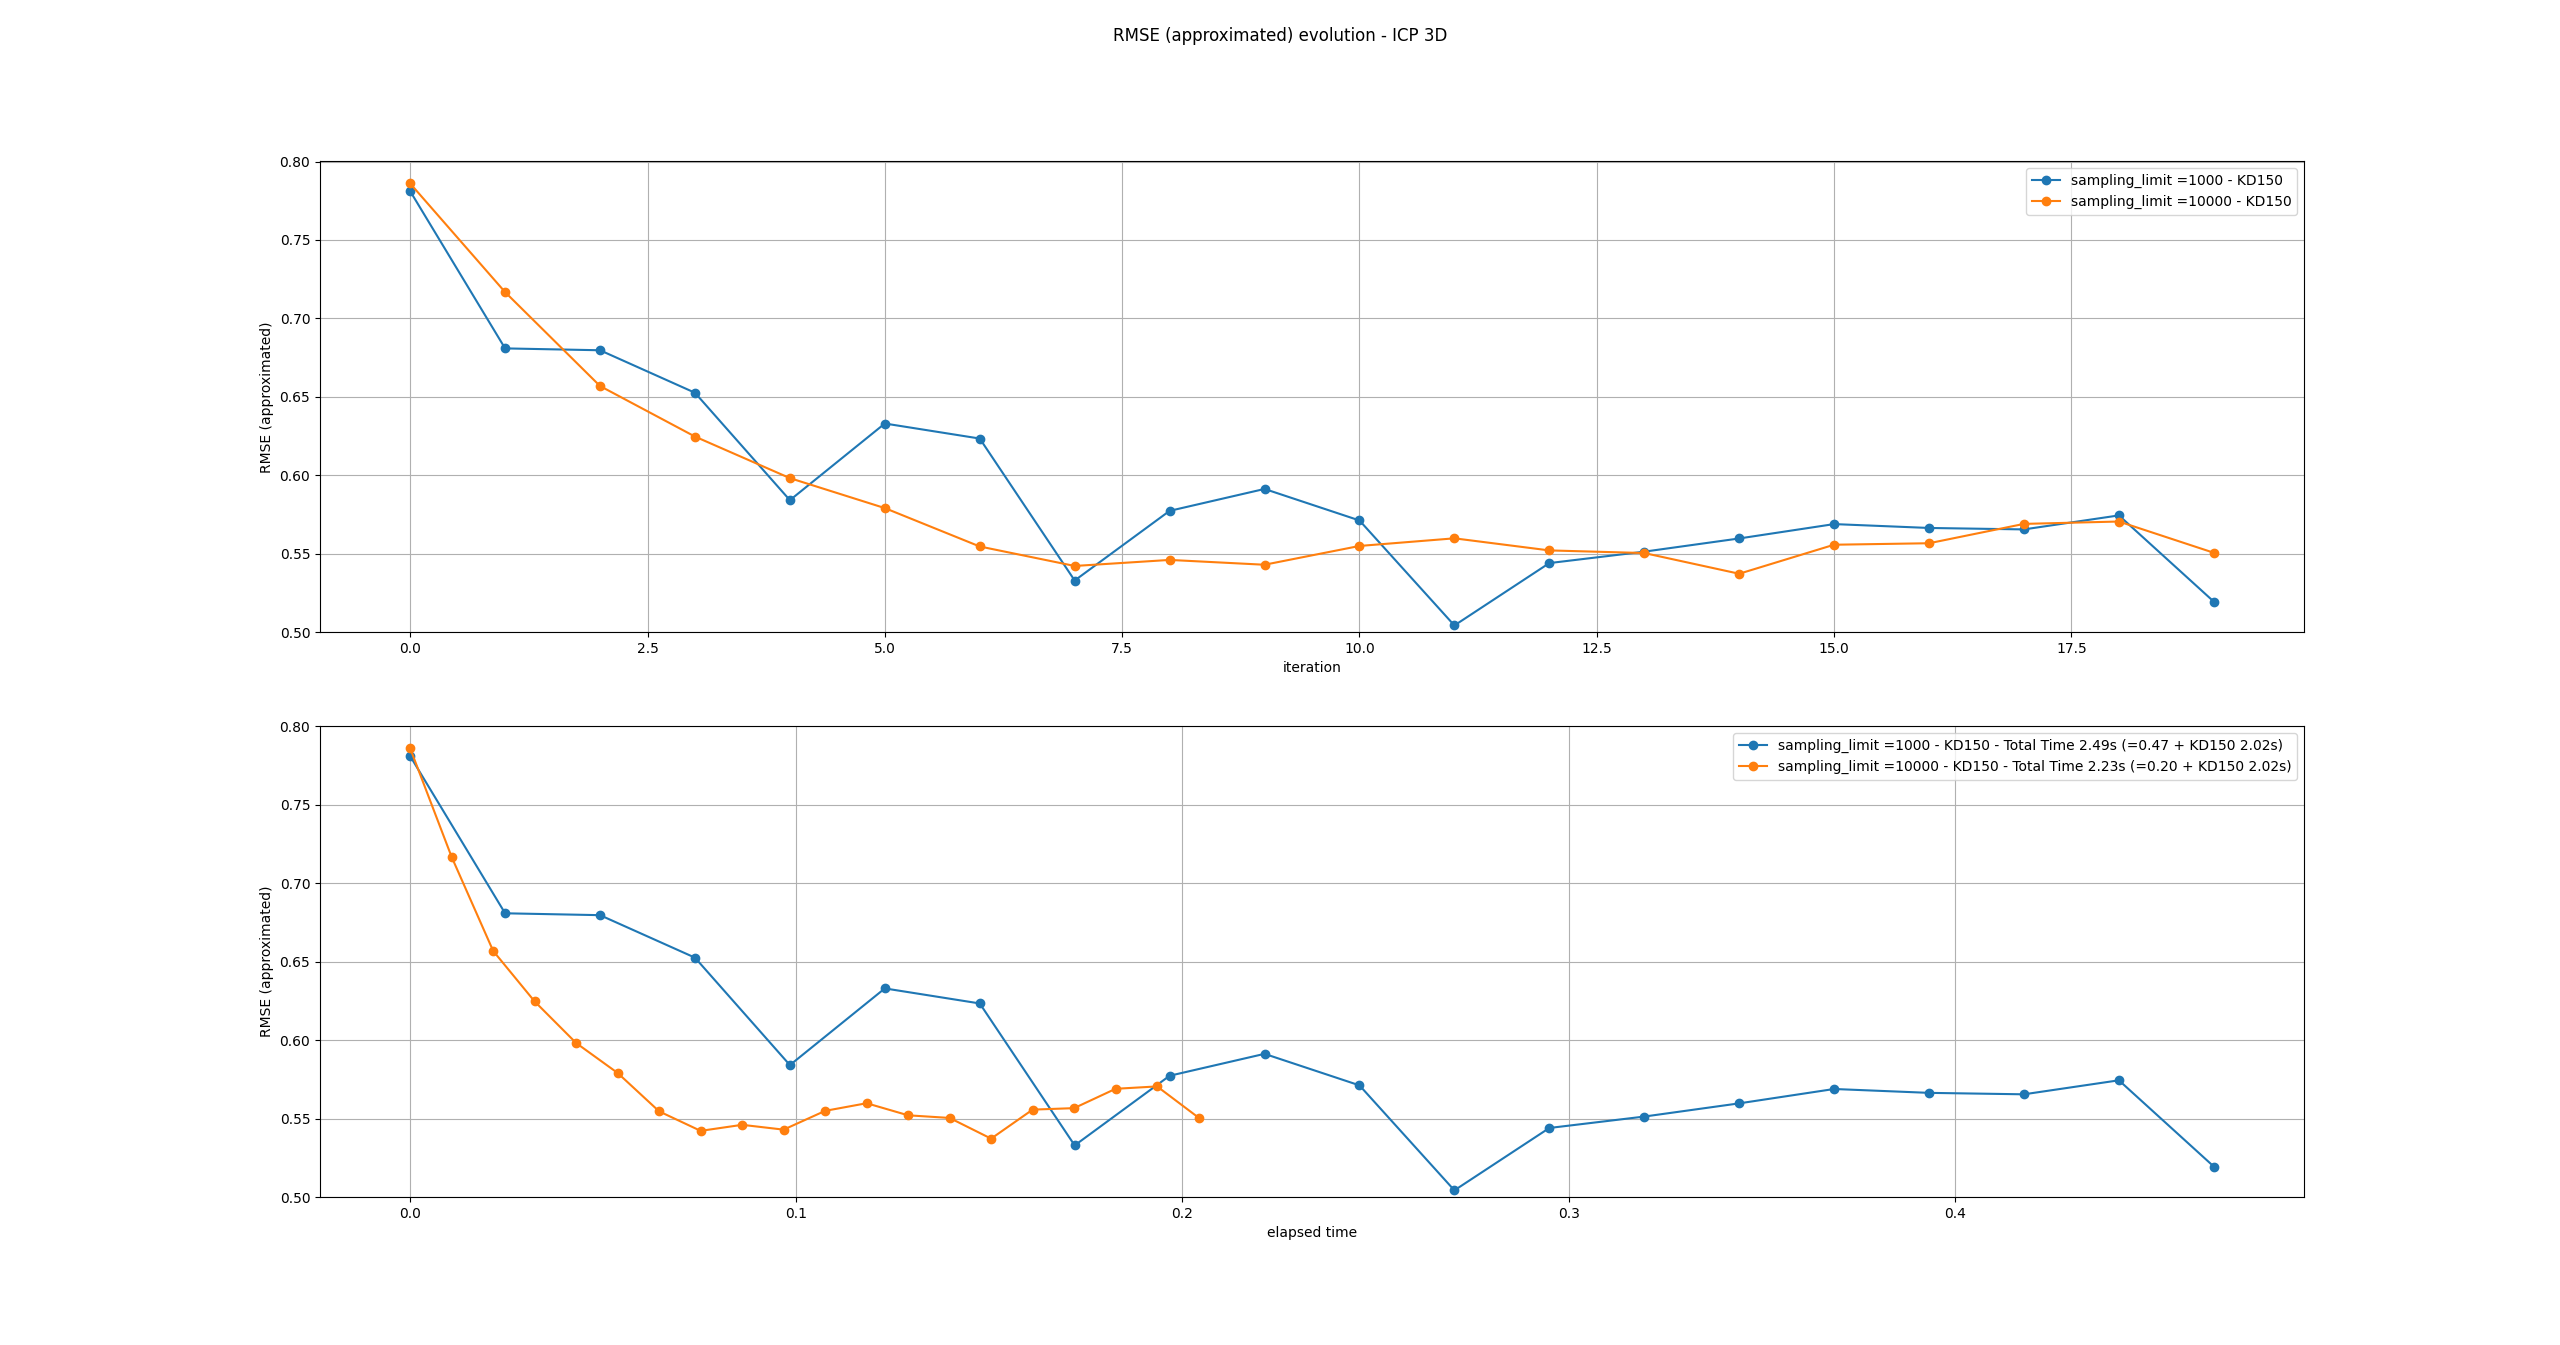
\includegraphics[width=1.\linewidth]{figures/RMS_APPROX_random_sampling_limit_1k_vs_10k.png}
  \caption{Evolution of the RMSE approximated over 1000 and  10.000 matched points. This would be the criterion to decide if the algorithm has converged. Top: horizontal axis is the number of iterations. Bottom: horizontal axis is the time spent in the registration, KD tree construction is ommitted but takes a few seconds.}
  \label{fig:real_scene_icp}
\end{figure}

\end{document}

